% !TeX~program = latexmk
% !TeX spellcheck = pl_PL
% !TeX~root = example.tex

\chapter{Jak korzystać z~szablonu pracy}

\textcolor{red}{
    Niniejszy rozdział zawiera prezentację możliwości przygotowanego szablonu pracy
    i zostanie usunięty we właściwej pracy.
}

Klasa przygotowana jest zgodnie z~zaleceniami dostępnymi ze strony \url{} i~może być wykorzystana do składu pracy \textbf{inżynierskiej} lub \textbf{magisterskiej} na wydziale mechanicznym.

Klasa zgodnie z~\href{http://www.wmech.pwr.wroc.pl/88428.dhtml}{wymaganiami Wydziału Mechanicznego} składa stronę tytułową i~stosuje się do zaleceń (czcionka, zasady numeracji, odstępy,\ldots).

Po raz pierwszy w~roku akademickim 2015/2016 prace dyplomowe będą sprawdzane przez program antyplagiatowy. Nie wiadomo jeszcze jakie to będzie miało konsekwencje dla prac składanych w~LaTeXu. Proponuję zaglądać do \href{http://kmim.wm.pwr.edu.pl/myszka/tag/antyplagiat/}{aktualności temu poświęconych}.

\section{Użycie}

\begin{enumerate}
\item
Praca magisterska i~inżynierska.

Wychodzi, że tak na prawdę powinny być dwie wersje pracy: do archiwum (marginesy 2,5 cm) i~„dla promotora”\footnote{Ciekawe po co mu…?}. Wersja dla promotora powinna mieć trochę większy margines od strony oprawy (35mm), najprawdopodobniej będzie drukowana \textbf{jednostronnie} i, żeby była łatwiejsza do czytania będzie złożona z~interlinią \textbf{1,5}.

Jak tak to tak:  pojawiły się dwie dodatkowe opcje klasy:
\begin{enumerate}
\item
\texttt{archiwum}: \verb|\usepackage[magister,archiwum]{dyplom}| — wersja do archiwum
\item
\texttt{druk}: \verb|\usepackage[inzynier,druk]{dyplom}| — wersja do „druku” (i oprawy).
\end{enumerate}
\textbf{W~przypadku braku opcji — wybierana jest wersja do archiwum!}

Tak na prawdę, to w~przypdku braku opcji powinna być wybierana wersja druk. Wybrałem jednak opisane wyzej zachowanie, aby zachowanie zmodyfikowanej klasy było zgodne z~dotychczasowym. Zalecam przeprowadzanie redakcji tekstu w~trybie druku i~pozostawienie dokumentu „jak wyjdzie” w~trybie archiwum. Chyba, że ilustracje będą zachowywać się bardzo dziwnie…

Ponieważ „doszły do mnie” jakieś dziwne informacje, że ze stroną tytułową jest coś nie tak, dokonałem kolejnych porównań. Różnica jest jedna: obecność ramki wokół tytułów pracy. W~związku z~tym, ramka została zlikwidowana. Można ją odzyskać dodając dodatkowy parametr: \verb|\usepackage[inzynier,druk,ramka]{dyplom}| i~się pojawi…
\item
Praca magisterska:
\begin{verbatim}
\documentclass[magister]{dyplom}
\end{verbatim}
Dodatkowo zdefiniować należy sposób kodowania polskich liter. W~przypadku systemu Windows będzie to najprawdopodobniej:
\begin{verbatim}
\usepackage[cp1250]{inputenc}
\end{verbatim}
a w~przypadku systemów linuksowych:
\begin{verbatim}
\usepackage[utf8]{inputenc}
\end{verbatim}

Dodatkowo zdefiniować należy „metadane”:
\begin{itemize}
\item
Nazwisko autora:
\begin{verbatim}
\author{Imię Nazwisko}
\end{verbatim}
\item
Tytuł pracy (w języku polskim):
\begin{verbatim}
\title{Tytuł Pracy}
\end{verbatim}
\item
Tytuł pracy po angielsku
\begin{verbatim}
\titlen{Work Title}
\end{verbatim}
\item
Nazwisko promotora
\begin{verbatim}
\promotor{prof. dr hab. inż. Imię Nazwisko, prof. PWr.}
\end{verbatim}
\item
Kierunek
\begin{verbatim}
\kierunek{Prawo}
\end{verbatim}
\item
Specjalność:
\begin{verbatim}
\specjalnosc{Lewo}
\end{verbatim}
\item
W~razię potrzeby wpisać można inną nazwę wydziału. Gdy nie zostanie wpisana — będzie tam Wydział Mechaniczny.
\begin{verbatim}
\wydzial{Wydział Elektryczny}
\end{verbatim}
\item
Praca może mieć konsultanta/konsultantów. Dodałem więc pole konsultant:
\begin{verbatim}
\konsultant{dr inż. Kazimierz Kabacki}
\end{verbatim}
Nazwisko konsultanta pojawi się miedzy nazwiskiem promotora a~oceną. Pozostaje kwestia czy powinien to być „konsultant” czy raczej „konsulktanci”?
\end{itemize}
Powyższe metadane umieszczamy przed \verb|\begin{document}|:
\begin{verbatim}
\documentclass[magister]{dyplom}
\usepackage[utf8]{inputenc}

\author{Jan A. Backi}
\title{Lorem ipsum dolor sit amet, consectetuer adipiscing elit}
\titlen{Lorem ipsum dolor sit amet, consectetuer adipiscing elit}
\promotor{dr hab. inż. Jerzy Babacki, prof. nadzw. PWr., I-77}
\wydzial{Wydział Mechaniczny}
\kierunek{Prawo}
\specjalnosc{Lewo}

\begin{document}
\end{verbatim}
\item
Praca inżynierska:
\begin{verbatim}
\documentclass[inzynier]{dyplom}
\end{verbatim}
Dodatkowo zdefiniować należy sposób kodowania polskich liter. W~przypadku systemu Windows będzie to najprawdopodobniej:
\begin{verbatim}
\usepackage[cp1250]{inputenc}
\end{verbatim}
a w~przypadku systemów linuksowych:
\begin{verbatim}
\usepackage[utf8]{inputenc}
\end{verbatim}

Dodatkowo zdefiniować należy „metadane”:
\begin{itemize}
\item
Nazwisko autora:
\begin{verbatim}
\author{Imię Nazwisko}
\end{verbatim}
\item
Tytuł pracy (w języku polskim):
\begin{verbatim}
\title{Tytuł Pracy}
\end{verbatim}
\item
Tytuł pracy po angielsku
\begin{verbatim}
\titlen{Work Title}
\end{verbatim}
\item
Nazwisko promotora
\begin{verbatim}
\promotor{prof. dr hab. inż. Imię Nazwisko, prof. PWr.}
\end{verbatim}
\item
Kierunek
\begin{verbatim}
\kierunek{Prawo}
\end{verbatim}
%\item
%Specjalność:
%\begin{verbatim}
%\specjalnosc{Lewo}
%\end{verbatim}
\item
W~razię potrzeby wpisać można inną nazwę wydziału. Gdy nie zostanie wpisana — będzie tam Wydział Mechaniczny.
\begin{verbatim}
\wydzial{Wydział Elektryczny}
\end{verbatim}
\item
Praca może mieć konsultanta/konsultantów. Dodałem więc pole konsultant:
\begin{verbatim}
\konsultant{dr inż. Kazimierz Kabacki}
\end{verbatim}
Nazwisko konsultanta pojawi się miedzy nazwiskiem promotora a~oceną. Pozostaje kwestia czy powinien to być „konsultant” czy raczej „konsultanci”?

\end{itemize}
Powyższe metadane umieszczamy przed \verb|\begin{document}|:
\begin{verbatim}
\documentclass[magister]{dyplom}
\usepackage[utf8]{inputenc}

\author{Jan A. Backi}
\title{Lorem ipsum dolor sit amet, consectetuer adipiscing elit}
\titlen{Lorem ipsum dolor sit amet, consectetuer adipiscing elit}
\promotor{dr hab. inż. Jerzy Babacki, prof. nadzw. PWr., I-77}
\wydzial{Wydział Mechaniczny}
\kierunek{Prawo}
\specjalnosc{Lewo}

\begin{document}
\end{verbatim}

\end{enumerate}

\section{Dodatkowe zasoby}

Warto wspomnieć  o~innych inicjatywach przyswojenia LaTeX{}a piszącym prace dyplomowe. Najważniejsza z~nich to książka Tomasza Przechlewskiego\nolink{tp-11-latex} oraz przygotowana przez niego klasa znajdująca się w~\url{https://github.com/hrpunio/wzmgr}. Przykłady z~książki znaleźć można w~\url{https://github.com/hrpunio/pmdzpl}.


\section{Ala ma kota}

ĄĆĘŁŃÓŚŹŻ ąćęłńóśźż\footnote{Przykład użycia polskich znaków diakrytycznych oraz przypisu w~miejscu}. \lipsum[1]

\section{Odniesienie do pozycji z~literatury (strona WWW)}

% Odniesienie do rysunku i~cytowanie dokumentu. Dokumenty są definiowane w~pliku literatura.bib
Reszta dokumentacji znajduje się w\nolink{docker_compose_reference}. \lipsum[3]

\section{Odniesienie do książki}

Jak pisze Harel w\nolink{harel_rzecz_2008}: \lipsum[7]

\section{Rysunek}

% Rysunek
\begin{figure}
    \centering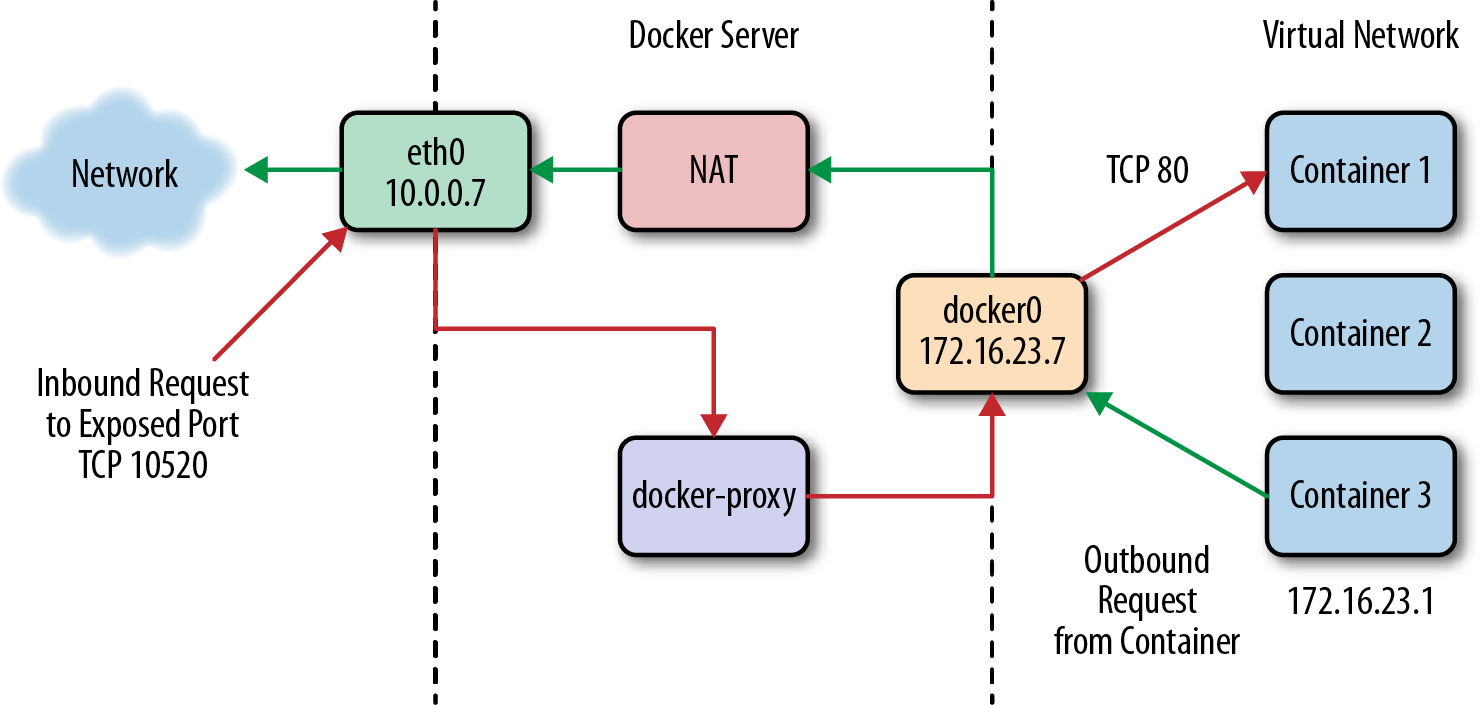
\includegraphics[width=.6\textwidth]{demo/img/swarm-network}
    \caption{Docker ma sieć}  \label{rys:network}
    \raggedright\source{\bibentry{docker_compose_reference}\nolink{docker_compose_reference}}
    % Źródło rysunku i~etykieta przez którą odwołujemy się do rysunku.
\end{figure}

Jak widać na rys. \ref{rys:network} Docker ma wewnętrzną sieć. \lipsum[1]


\subsection{Rysunek z~kotem}

Jak widać na rys.\ref{rysunek:kot} Ala ma kota. \lipsum[9-10]

\begin{figure}[H]
    \centering
\includegraphics[width=.4\textwidth]{demo/img/kotek}
    \caption{Ala ma kota}\label{rysunek:kot}
    \raggedright\source{\ownwork}
\end{figure}

\subsection{Tabela}

Co uwzględniono w~tabeli \ref{tabela:coktoma}. \lipsum[13-15]

% Tabela. Nazwa tabeli u~góry.
\begin{table}[h!]
    \raggedright\caption{Co kto ma (patrz też dodatek~\ref{app:dod1}) \label{tabela:coktoma}}
    \begin{center}\begin{tabular}{|l|l|l|}% wyrównanie kolumn tabeli -> l~c r~- do lewej, środka, do prawej
        \hline
        Ala & ma & kota \\
        \hline
        Ola & ma & psa \\
        \hline
        Ula & ma & małpę\\
        \hline
    \end{tabular}\end{center}


    \raggedright\source{\bibentry{harel_rzecz_2008}\nolink{harel_rzecz_2008}}
\end{table}

\lipsum[19-20] Warto wspomnieć, że w\nolink{aizawa_groundwater_2009} rzecz przedstawiona jest zupełnie inaczej. Poniższy wzór:

\begin{equation}
    \sum_{i=1}^{\infty}a_i
    \label{eq:mojWzor}
\end{equation}

Wzór \ref{eq:mojWzor} wskazuje że dowód podany w\nolink{kaleta_experimental_2005} może zostać podważony. \lipsum[9]

\section{Kod źródłowy}

% lub {java} albo {bash} albo {text}
\begin{listing}[h!]
    \caption{Przykładowy algorytm w~języku C} \label{listing:moj}
    \begin{minted}{c}
        int main()
        {
        int a=2*3;
        printf("**Ala ma kota\n**");
        while(!I2C_CheckEvent(I2C1, I2C_EVENT_MASTER_MODE_SELECT)); /* EV5 */
        return 0;
        }
    \end{minted}
    \raggedright\source{\ownwork}
\end{listing}

W~moim kodzie \ref{listing:moj} zrobiłem coś wspaniałego. \lipsum[4]

% !TeX spellcheck = pl_PL
\section{Przydatne sztuczki}
\section{Makra dodane w szablonie}
\begin{enumerate}
    \item source - służy do definiowania źródła obrazka, tabeli czy listingu

%    \begin{verbatim}
%\source{github.com}
%# (źródło: github.com)
%    \end{verbatim}

    \item ownwork
    \item req
    \item atr
    \item capmystring
    \item role
    \item image
    \item imagewide
    \item todo
    \item inlinetodo
    \item cellred
    \item cellgreen
    \item cellgray
    \item listnormal
    \item mynobreakpar
    \item threedigits
    \item twodigits

\end{enumerate}


\section{Przykłady tabel}

\begin{minipage}{\textwidth}
    \begin{table}[H]
        \raggedright\caption{Rozwiązania konkurencyjne~- cechy funkcjonalne\label{tabela:rozwiazania-konkurencyjne-funkcjonalne}}
        \begin{center}\begin{tabular}{|P{.22\textwidth}|P{.09\textwidth}|P{.09\textwidth}|P{.09\textwidth}|P{.09\textwidth}|P{.09\textwidth}|P{.09\textwidth}|}
            \hline
            & \cellgray{Rozw1}      & \cellgray{Rozw2}          & \cellgray{Rozw3}         & \cellgray{Rozw4}           & \cellgray{Rozw5}      & \cellgray{Rozw6}    \\ \hline
            \cellgray{Funkcjonalność 1}        & \cellgreen{TAK}       & \cellgreen{TAK}           & \cellgreen{TAK}          & \cellgreen{TAK}            & \cellgreen{TAK}       & \cellgreen{TAK}     \\ \hline
            \cellgray{Funkcjonalność 2}        & \cellgreen{TAK}       & \cellgreen{TAK}           & \cellgreen{TAK}          & \cellgreen{TAK}            & \cellred{NIE}         & \cellred{NIE}       \\ \hline
            \cellgray{Funkcjonalność 3}        & \cellgreen{TAK}       & \cellgreen{TAK}           & \cellgreen{TAK}          & \cellgreen{TAK}            & \cellgreen{TAK}       & \cellgreen{TAK}     \\ \hline
            \cellgray{Funkcjonalność 4}        & \cellgreen{TAK}       & \cellgreen{TAK}           & \cellgreen{TAK}          & \cellgreen{TAK}            & \cellred{NIE}         & \cellgreen{TAK}     \\ \hline
            \cellgray{Funkcjonalność 5}        & \cellgreen{TAK}       & \cellgreen{TAK}           & \cellgreen{TAK}          & \cellred{NIE}              & \cellred{NIE}         & \cellgreen{TAK}     \\ \hline
            \cellgray{Funkcjonalność 6}        & \cellgreen{TAK}       & \cellgreen{TAK}           & \cellgreen{TAK}          & \cellgreen{TAK}            & \cellgreen{TAK}       & \cellgreen{TAK}     \\ \hline
            \cellgray{Funkcjonalność 7}        & \cellgreen{TAK}       & \cellgreen{TAK}           & \cellgreen{TAK}          & \cellred{NIE}              & \cellgreen{TAK}       & \cellgreen{TAK}     \\ \hline
            \cellgray{Funkcjonalność 8}        & \cellgreen{TAK}       & \cellgreen{TAK}           & \cellgreen{TAK}          & \cellgreen{TAK}            & \cellgreen{TAK}       & \cellred{NIE}       \\ \hline
            \cellgray{Funkcjonalność 9}        & \cellgreen{TAK}       & \cellgreen{TAK}           & \cellgreen{TAK}          & \cellgreen{TAK}            & \cellgreen{TAK}       & \cellgreen{TAK}     \\ \hline
            \cellgray{Funkcjonalność 10}       & \cellgreen{TAK}       & \cellgreen{TAK}           & \cellgreen{TAK}          & \cellgreen{TAK}            & \cellgreen{TAK}       & \cellgreen{TAK}     \\ \hline
        \end{tabular}\end{center}
        \raggedright\source{\ownwork}
    \end{table}
\end{minipage}

\begin{minipage}{\textwidth}
    \begin{table}[H]
        \raggedright\caption{Sformułowanie problemu\label{tabela:sformulowanie-problemu}}
        \begin{center}\begin{tabular}{|P{.2\textwidth}|p{.7\textwidth}|}

            \hline
            \cellgray{Problem} &
            \inlinetodo{todo} \\
            \hline

            \cellgray{Dotyczy} &
            \inlinetodo{todo} \\
            \hline

            \cellgray{Wpływ problemu} &
            \begin{itemize}
                \item \inlinetodo{todo}
                \item \inlinetodo{todo}
                \item \inlinetodo{todo}
            \end{itemize} \\
            \hline

            \cellgray{Pomyślne rozwiązanie} &
            \begin{itemize}
                \item \inlinetodo{todo}
                \item \inlinetodo{todo}
                \item \inlinetodo{todo}
            \end{itemize} \\
            \hline
        \end{tabular}\end{center}
        \raggedright\source{\ownwork}
    \end{table}
\end{minipage}

\begin{minipage}{\textwidth}
    \begin{table}[H]
        \raggedright\caption{Użytkownicy\label{tabela:uzytkownicy}}
        \begin{center}\begin{tabular}{|P{.15\textwidth}|P{.25\textwidth}|P{.5\textwidth}|}

            \hline
            \cellgray{Nazwa} & \cellgray{Opis} & \cellgray{Odpowiedzialności}\\

            \hline
            Gość &
            Niezalogowany użytkownik &
            \begin{itemize}
                \item Zakłada konto użytkownika.
                \item Wyświetla stronę główną.
            \end{itemize} \\
            \hline
            Administrator &
            Osoba zarządzająca działaniem aplikacji &
            \begin{itemize}
                \item Przydzielanie i~odbieranie użytkownikom uprawnień.
                \item Zarządzanie definicjami wartości odżywczych, typami diet, typami posiłków, typami dań i~wyposażeniem kuchennym.
            \end{itemize} \\
            \hline
        \end{tabular}\end{center}
        \raggedright\source{\ownwork}
    \end{table}
\end{minipage}

\section{Przykłady numerowania}
\subsection{Słownik pojęć domenowych}\label{sec:dictionary}
Na podstawie rozważań z~rozdziału \ref{ch:knowladge-state} sporządzono następującą listę definicji domenowych istotną z~punktu widzenia projektu:
\begin{itemize}[series=atr, wide, align=left, leftmargin=190pt]
    \atr{BIA}- metoda impedancji bioelektrycznej wykorzystywana do analizy składu ciała
    \atr{BMI}- wskaźnik masy ciała
    \atr{CPM}- całkowita przemiana materii
\end{itemize}
\subsection{Kategorie}\label{subsec:database:categories}

\begin{enumerate}[label={\textbf{KAT/\protect\threedigits{\theenumi}}}, wide, labelwidth=!, labelindent=0pt, labelsep=0pt, series=reqs]
    \setlength\itemsep{1.75em}
    \req{User}\label{kat:User} (Użytkownik)\\
    \indent\textbf{Opis}: Konto użytkownika aplikacji. Każdy zalogowany użytkownik musi mieć konto użytkownika.
    \par
    \textbf{Atrybuty}:
    \begin{itemize}[series=atr, wide, align=left, leftmargin=190pt]
        \atr{id}\label{kat:User:id}- identyfikator
        \atr{login}\label{kat:User:login}- login użytkownika
        \atr{passwordHash}\label{kat:User:passwordHash}- reprezentacja hasła utworzona przez nałożenie na hasło funkcji skrótu
    \end{itemize}

    \req{Authority}\label{kat:Authority} (Rola)\\
    \indent\textbf{Opis}: Rola użytkownika od której zależy zakres uprawnień użytkownika.
    \par
    \textbf{Atrybuty}:
    \begin{itemize}[series=atr, wide, align=left, leftmargin=190pt]
        \atr{name}\label{kat:Authority:name}- nazwa roli
    \end{itemize}
\end{enumerate}

\subsection{Reguły funkcjonowania}\label{subsec:database:functionalRules}

\begin{itemize}[label={\textbf{Reguły dla}}, wide, labelwidth=!, labelindent=0pt]
    \setlength\itemsep{1.75em}
    \item\ref{kat:User}\mynobreakpar
    \begin{enumerate}[label={\textbf{REG/\protect\threedigits{\arabic{enumi}}}}, wide, labelwidth=!, align=left, leftmargin=3cm]
        %Relacje
        \item Użytkownik (\ref{kat:User}) musi mieć przynajmniej jedną rolę (\ref{kat:Authority}).
        \item Użytkownik (\ref{kat:User}) może mieć wiele ról (\ref{kat:Authority}).
        %CRUD
        \item \role{Gość} może dodawać nowego użytkownika (\ref{kat:User}).
        \item \role{Użytkownik} może wyświetlać, edytować i~usuwać swoje dane użytkownika (\ref{kat:User}).
        \item \role{Administrator} może wyświetlać i~usuwać dane użytkownika (\ref{kat:User}).
    \end{enumerate}
    \item\ref{kat:Authority}\mynobreakpar
    \begin{enumerate}[label={\textbf{REG/\protect\threedigits{\arabic{enumi}}}}, wide, labelwidth=!, align=left, leftmargin=3cm, resume]
        %Relacje
        %CRUD
        \item \role{Administrator} może dodawać, wyświetlać, edytować i~usuwać dane roli (\ref{kat:Authority}).
    \end{enumerate}
\end{itemize}

\subsection{Ograniczenia dziedzinowe}\label{subsec:database:restrictions}

\begin{itemize}[label={\textbf{Ograniczenia dla}}, wide, labelwidth=!, labelindent=0pt]
    \setlength\itemsep{1.75em}
    \item\ref{kat:User}\mynobreakpar
    \begin{enumerate}[label={\textbf{OGR/\protect\threedigits{\arabic{enumi}}}}, wide, labelwidth=!, align=left, leftmargin=3cm]
        %Required
        \item Atrybut \ref{kat:User:login} jest wymagany.
        \item Atrybut \ref{kat:User:passwordHash} jest wymagany.
        %Unique
        \item Atrybut \ref{kat:User:login} ma unikalną wartość.
        %Type
        \item Atrybut \ref{kat:User:login} jest ciągiem znaków składającym się z~liter, cyfr i~dodatkowo mogącym zawierać znaki ".", "\_", "-", "@" o~długości od 1~do 50 znaków.
        \item Atrybut \ref{kat:User:passwordHash} jest ciągiem znaków o~długości 60 znaków.
    \end{enumerate}
    \item\ref{kat:Authority}\mynobreakpar
    \begin{enumerate}[label={\textbf{OGR/\protect\threedigits{\arabic{enumi}}}}, wide, labelwidth=!, align=left, leftmargin=3cm, resume]
        \item Atrybut \ref{kat:Authority:name} jest wymagany.
        \item Atrybut \ref{kat:Authority:name} ma unikalną wartość.
        \item Atrybut \ref{kat:Authority:name} jest ciągiem znaków składającym się z~liter i~znaków "\_" o~długości od 1~do 255 znaków.
    \end{enumerate}

\end{itemize}

%\section{Przykład kodu}
%\noindent\hspace{.075\textwidth}\begin{minipage}{.85\textwidth}
%                                    \begin{minted}{java}
%/**
%* Short description of measure in language of a~product, e.g. \"cup\" or \"tea spoon\"
%*/
%@NotNull
%@Size(min = 1, max = 255)
%private String description;
%                                    \end{minted}
%                                    \begin{lstlisting}[caption={Komentarz w~stylu JavaDoc \source{\ownwork}}, label={listing:javadoc}]
%                                    \end{lstlisting}
%\end{minipage}
\thispagestyle{normal}
